\documentclass[11pt]{article}
\usepackage{geometry}
\usepackage{graphicx}
\usepackage{enumitem}
\usepackage{float}
\usepackage{amsmath}
\usepackage{multicol}
\usepackage{cancel}
\usepackage{mathrsfs}

\geometry{a4paper, top=0.5in, bottom=0.5in, right=0.75in, left=0.75in}

\title{Lecture 6}
\author{}
\date{}

\begin{document}

\maketitle

\section{Gain Saturation}
\begin{itemize}
    \item For oscillation, we have to satisfy the phase condition ($\nu = \frac{qc}{2L}$), so only longitudinal modes are allowed. Also, we have to satisfy the gain condition ($\gamma > \alpha_s + \frac{1}{2L} \ln \left( \frac{1}{R_1 R_2} \right)$).
    \item During operation, we lose some of the population inversion and the gain curve moves down until it reaches steady state. At steady state, only the modes that satisfy the gain condition will oscillate.
    \item Settling means that the gain is equal to $\alpha_r$ at the oscillating frequency.
\end{itemize}

\subsection{Homogeneous Broadening}

If the center of the Lorentzian ($\nu_o$) coincides with one of the longitudinal modes, only $\nu_o$ will oscillate. 
\begin{center}
    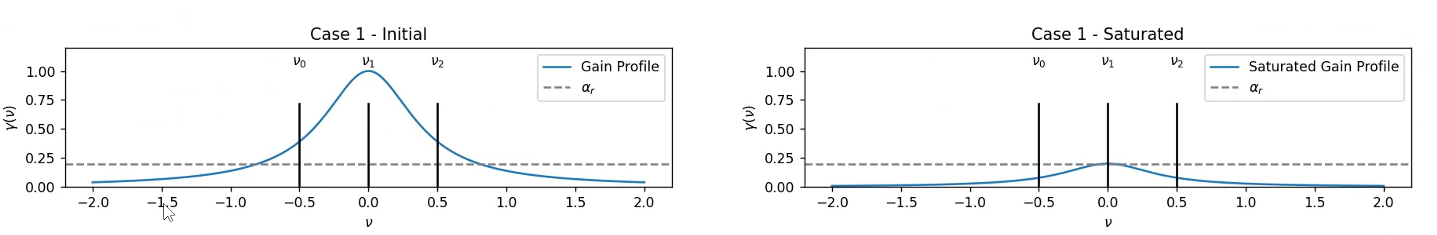
\includegraphics[scale=0.55]{1.png}
\end{center}
If the center of the Lorentzian ($\nu_o$) does not coincide with one of the longitudinal modes AND the longitudinal modes are not symmetrically distributed around $\nu_o$, the closest mode to $\nu_o$ will oscillate.
\begin{center}
    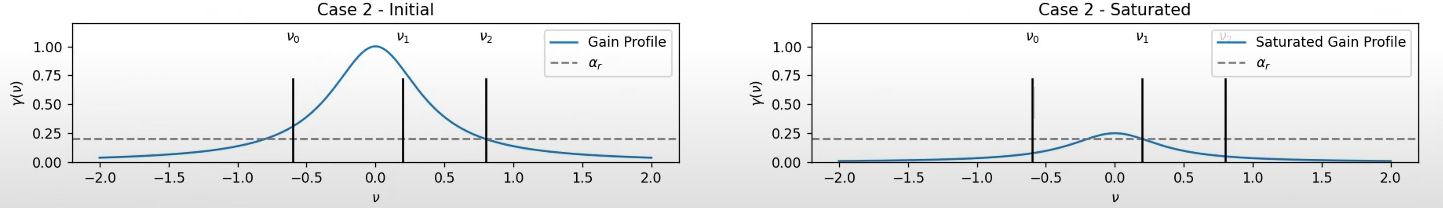
\includegraphics[scale=0.55]{2.png}
\end{center}
If the center of the Lorentzian ($\nu_o$) does not coincide with one of the longitudinal modes AND the longitudinal modes are symmetrically distributed around $\nu_o$, both modes around $\nu_o$ will oscillate.
\begin{center}
    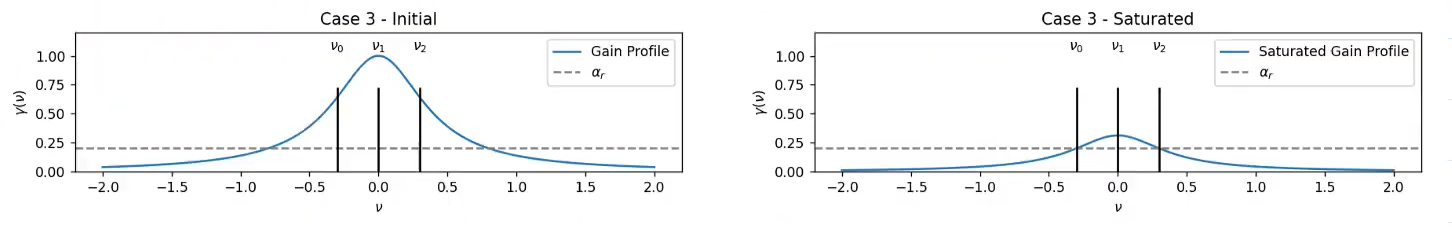
\includegraphics[scale=0.55]{3.png}
\end{center}
\textbf{Note:} In semiconductor lasers, PIN has a waveguide structure, so there are transverse modes as well. 
\begin{center}
    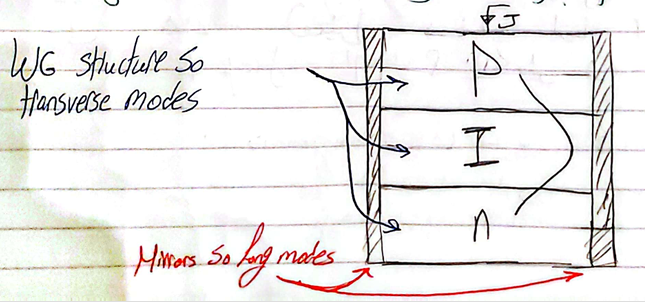
\includegraphics[scale=0.55]{5.png}
\end{center}

\subsection{Inhomogeneous Broadening}
Recall that each group of atoms has a Lorentzian gain curve, but overall the gain curve is Gaussian. As population inversion decreases, the gain curve moves down for each group of atoms at the longitudinal modes, so we notice some dips in the overall Gaussian gain curve. 
\begin{center}
    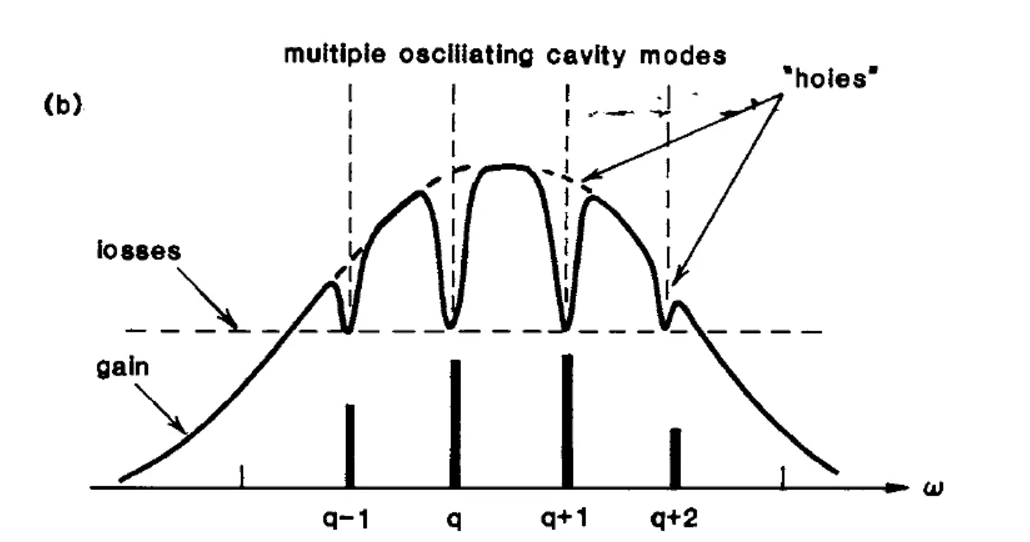
\includegraphics[scale=0.5]{4.png}
\end{center}
\begin{itemize}
    \item For inhomogenous broadening, all longitudinal modes that initially satisfy the gain condition will oscillate.
    \item For inhomogenous broadening, the number of oscillating modes is $\frac{B}{\nu_F}$, where $B$ is the gain bandwidth (where $\gamma > \alpha_r$) and $\nu_F$ is the free spectral range.
    \item The output power for each resonnaing mode is different which leads to mode competition.
    \item Inhomogeneous broadening oscillate at multiple frequencies even if $\nu_o$ coincides with a longitudinal mode.
    \item For ideal LASER, the output frequency, amplitude, and phase are constant.
\end{itemize}

\subsection{Space Dependance}
\begin{itemize}
    \item Inside the LASER cavity, we have a standing wave, so at certain points we have $\phi_{max}$, so gain saturation occurs, while at other points we have $\phi_{min}$ and gain saturation does not occur. This is called spatial hole burning.
    \item $\gamma = \frac{\sigma N_o}{1 + \frac{\phi}{\phi_s}}$, where $\phi$ is a function in space.
    \item If $R_1 = R_2 = 1$, the standing wave is from $0$ to $\phi_{max}$.
    \item If $R < 1$, the standing wave is between $\phi_{min}$ to $\phi_{max}$.
    \item The problem with spatial hole burning is that the points with $\phi_{min}$ will never change when changing $\phi_{in}$, and no gain saturation will occur at these points, so multiple modes will oscillate (even in ideal homogeneous broadening).
    \item Note that the longitudinal modes are not a perfect impulse and have bandwidth ($\nu_q + \Delta \nu$) due to cavity losses.
    \item Therefore, the output is not monochromatic even if we do not have spatial hole burning.
\end{itemize}

\section{LASER Oscillator}
To get oscillation $\rightarrow \gamma = \alpha_r$:
\begin{align*}
    \frac{\sigma N_o}{1 + \frac{\phi}{\phi_s}} = \alpha_r \rightarrow \frac{\phi}{\phi_s} = \frac{\sigma N_o}{\alpha_r} - 1 \\
    \phi = \phi_s \left( \frac{\sigma N_o}{\alpha_r} - 1 \right) = \phi_s \left( \frac{\gamma_o}{\alpha_r} - 1 \right)
\end{align*}
As gain decreases, $\phi$ decreases, which explains why in inhomogenous broadening, the frequencies with small $g(\nu)$ will have small $\phi$.
\begin{center}
    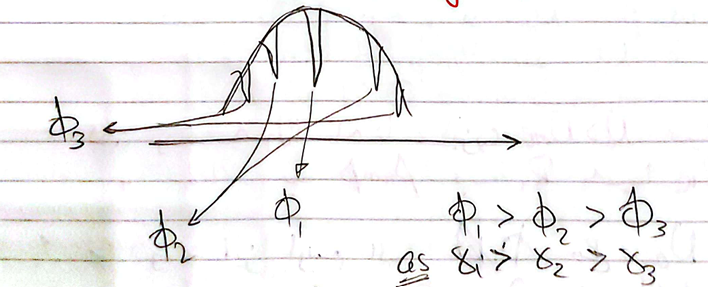
\includegraphics[scale=0.8]{6.png}
\end{center}
\textbf{Notes:} 
\begin{itemize}
    \item If $\gamma_o >> \alpha_r$, the line has large power, so output power depends on the difference between $\gamma_o$ and $\alpha_r$.
    \item We have to pump till $\gamma > \alpha_r$, as nonlinearity will decrease $\gamma$ until it reaches $\alpha_r$.
\end{itemize}
Threshold condition: $\gamma_{o_{th}} = \alpha_r$:
\begin{align*}
    \sigma N_o = \alpha_r \rightarrow N_{o_{th}} = \frac{\alpha_r}{\sigma}
\end{align*}
$N_{o_{th}}$ indicates $R_{th}$ as there is a relation between them obtained from the rate equations. \\ \\
\textbf{To draw $\phi$ vs $N_o$:}
\begin{itemize}
    \item If $N_o < N_{o_{th}} \rightarrow \gamma_o < \alpha_r$, no oscillation and LASER output is zero (ignoring spontaneous emission).
    \item If $N_o = N_{o_{th}}$, oscillation starts and $\phi = \phi_s \left( \frac{\sigma N_o}{\alpha_r} - 1 \right)$.
\end{itemize}
\begin{center}
    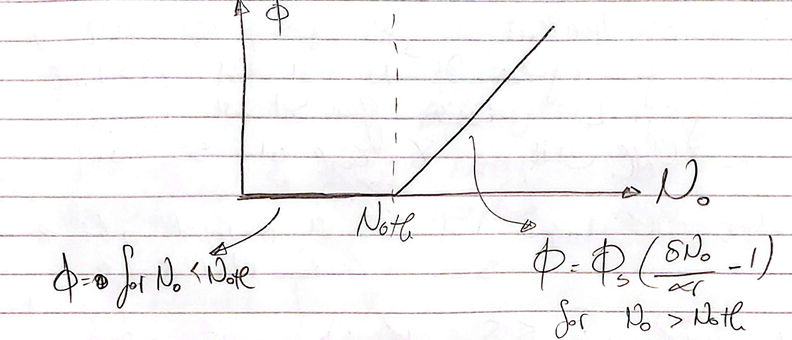
\includegraphics[scale=0.8]{7.png}
\end{center}
\textbf{To draw $N$ vs $N_o$:}
\begin{itemize}
    \item If $N_o < N_{o_{th}}$, there is no oscillation, so there is no effect on $N$, so $N = N_o$.
    \item If $N_o > N_{o_{th}}$, there is oscillation. From transient POV, $N$ should decrease due to gain saturation till it reaches $N_{o_{th}}$, so from steady state POV, $N = N_{o_{th}}$.
\end{itemize}
\begin{center}
    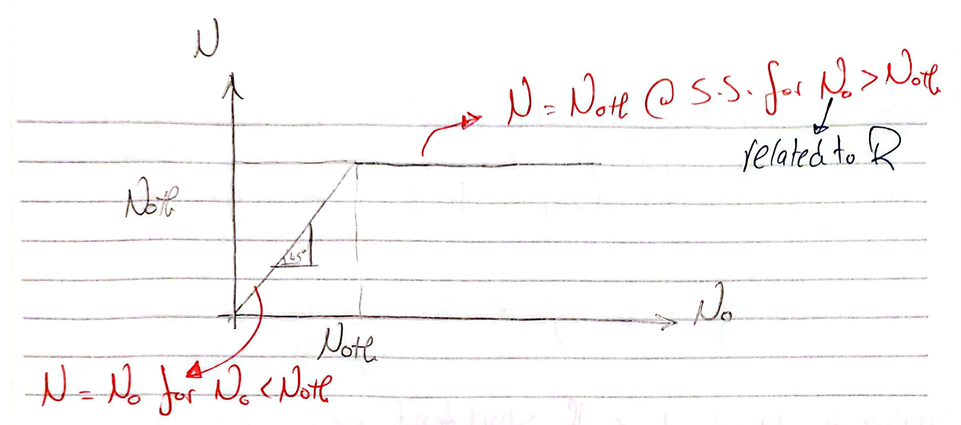
\includegraphics[scale=0.8]{8.png}
\end{center}

\subsection{Power Analysis}

\begin{align*}
    \phi &= \frac{\text{\# atoms}}{\text{area . time}} \rightarrow \phi h \nu = \frac{\text{energy}}{\text{area . time}} = \frac{\text{power}}{\text{area}} = I \\
    I_{out} &= \phi h \nu T
\end{align*}
where $T$ is the power reflection coefficient of the output mirror. \\ \\
\textbf{Notes:}
\begin{itemize}
    \item LASER is a gain medium between 2 mirrors, so we make 1 of the mirrors fully reflective and the other partially reflective to obtain output.
    \item We usually select mirrors with a very close power reflectivity (100\% and 97\%). This helps us make this approximation: $\phi^+ \approx \phi^- \approx \frac{\phi}{2}$.
\end{itemize}
\begin{center}
    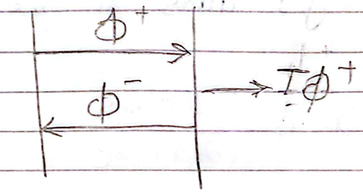
\includegraphics[scale=0.8]{9.png}
\end{center}
\begin{align*}
    I_{out} &= \frac{T}{2} \phi h \nu =  \frac{T}{2} \phi_s \left( \frac{\sigma N_o}{\alpha_r} - 1 \right) h \nu
\end{align*}
\textbf{Notes:}
\begin{itemize}
    \item If $R_1 = R_2 \rightarrow \phi^+ = \phi^-$, so we have a pure standing wave. If $R_1 \neq R_2 \rightarrow \phi^+ \neq \phi^-$, so we have both standing and travelling waves.
    \item As $R$ increases, $\alpha_r$ decreases, so it is better to use mirrors with high reflectivity to have a smaller threshold.
    \item However, if reflectivity increases, transmission decreases, so we have a smaller output power.
    \item There is a trade-off between decreasing cavity losses and increasing output power.
    \item To get the optimum point, we will differentiate $I_{out}$ with respect to $T$ and set it to zero.
\end{itemize}

\begin{align*}
    \alpha_r &= \alpha_s + \frac{1}{2L} \ln \left( \frac{1}{R_1 R_2} \right)
\end{align*}
Let $R_1 = R_2 = R = 1 - T$:
\begin{align*}
    \alpha_r &= \alpha_s - \frac{1}{2L} \ln(1 - T)
\end{align*}
$ln(1+x) \approx x$ if $x << 1$:
\begin{align*}
    \alpha_r &= \alpha_s - \frac{1}{2L} (-T) = \frac{2 \alpha_s L + T}{2L}
\end{align*}
So:
\begin{align*}
    I_{out} &= \frac{h \nu \phi_s}{2} \left( \frac{\gamma_o}{\alpha_r} - 1 \right) T \\
    &= \frac{h \nu \phi_s}{2} \left( \frac{2\gamma_o L}{2 \alpha_s L + T} - 1 \right) T \\ 
\end{align*}
Let $g_o = 2\gamma_o L$ and $\mathscr{L} = 2 \alpha_s L$:
\begin{align*}
    I_{out} &= \frac{h \nu \phi_s}{2} \left( \frac{g_o T}{\mathscr{L} + T} - T \right)
\end{align*}
Differentiate $I_{out}$ with respect to $T$ and set it to zero:
\begin{align*}
    \frac{\partial I_{out}}{\partial T} &= \frac{h \nu \phi_s}{2} \left[ \frac{(\mathscr{L} + T)g_o - g_o T}{(\mathscr{L} + T)^2} - 1 \right]  \\
    &= \frac{h \nu \phi_s}{2} \left[ \frac{\mathscr{L}g_o}{(\mathscr{L} + T)^2} \right] = 0 
\end{align*}
So:
\begin{align*}
    \mathscr{L}g_o = (\mathscr{L} + T)^2 \Rightarrow T = \sqrt{\mathscr{L}g_o} - \mathscr{L}
\end{align*}

\end{document}